\documentclass{article}
\usepackage{tikz}
\usetikzlibrary{angles, quotes}
\usepackage{amssymb}
\usepackage{pgfplots}
\pgfplotsset{width=10cm,compat=1.9}
\usepgfplotslibrary{statistics}
\usepackage[left=2.54cm,right=2.54cm,top=2.54cm,bottom=2.54cm]{geometry}
\usepackage{tasks} %Paquete necesario para la producción de items horizontales para algunos ejercicios de tarea empleando el comando /begin{multicols}}{#}.../end{multicols} para ayudarnos a reducir las páginas
\usepackage{pdflscape} %comando que permite cambiar a orientación horizontal las hojas%
\usepackage{soul} %Paquete para permitir la compilación de acentos usando el comando {\hl{}}}\\
\sethlcolor{yellow(munsell)} %comando para definir el color para el subrayado usando el comando \hl
\usepackage[utf8]{inputenc}
\usepackage[spanish]{babel}
\usepackage{icomma}
\usepackage{ragged2e}
\usepackage{siunitx}
\usepackage{url}
\usepackage[colorlinks=true, urlcolor=blue,  linkcolor=black, citecolor=green]{hyperref}
\usepackage{pdfpages}
\usepackage{blindtext} %Paquete que genera texto ficticio (dummy text) con el comando: \blindtext
\usepackage{cancel} %in the preamble gives you four different modes of striking through: \cancel{text to cancel} draws a diagonal line (slash) through its argument, \bcancel{text to cancel} uses the negative slope (a backslash), \xcancel{text to cancel} draws an X (actually \cancel plus \bcancel), \cancelto{〈value〉}{〈expression〉} draws a diagonal arrow through the 〈expression〉pointing to the 〈value〉 (math-mode only)
\usepackage{csquotes}
\usepackage{afterpage}
\usepackage{parskip} 
\usepackage{float}
\usepackage{enumitem}
\usepackage{multicol}%Paquete que permite la creación aislada de columnas de texto. De esta forma se reduce la cantidad de páginas en nuestro documento
\usepackage{lipsum} %Paquete que genera texto de relleno al igual que \usepackage{blindtext}, se usa con el comando \lipsum[#-#] los #(hashtags) delimitan el número de páginas que deseamos ocupar del paquete lipsum para usarlos como relleno. 

% Definir el comando personalizado para la nota
\newcommand{\mynote}[1]{%
\begin{tikzpicture}[baseline=-0.75ex]
	\node[draw, circle, fill=Apple Green!60, inner sep=2pt] (note) {\textbf{Nota:}};
\end{tikzpicture}%
\ \textit{#1}%
}

\newenvironment{Figura}
{\par\medskip\noindent\minipage{\linewidth}}
{\endminipage\par\medskip}
\usepackage{caption}
\usepackage[
backend=biber,
sorting=none,
url=true
]{biblatex} %bibliografía
\addbibresource{biblio.bib}
% Establecer el espacio entre las entradas de la bibliografía
\setlength{\bibitemsep}{1\baselineskip} % Puedes ajustar el valor según tus preferencias
\usepackage{amsmath,amsthm,amssymb,amsfonts}
\usepackage{pifont} %Permite la compilación del comando \xmark: es el símbolo de la tachita
\usepackage{mathtools} %permite la compilación de símbolos para matrices
\usepackage{empheq} %Paquete que se relaciona con \usepackage[most]{tcolorbox} para la creación de cuadros/cajas de colores para delimitar los resultados matemáticos o líneas de texto usando la línea de comando: \begin{empheq}[box={\mymath[colback=orange(webcolor)!70,drop lifted shadow]}]{equation*} \end{empheq}
\usepackage[most]{tcolorbox} %Paquete que se relaciona con \usepackage{empheq} para la creación de cuadros/cajas de colores para delimitar los resultados matemáticos o líneas de texto
\renewcommand{\qedsymbol}{$\blacksquare$}
\usetikzlibrary{positioning,decorations.pathreplacing} %Paquete que permite la compilación de llaves para cuadros sinópticos (brace diagram) 
\usepackage{schemata} %The schemata package is designed just for these brace diagrams
\usepackage{booktabs}

\newcommand\AB[2]{\schema{\schemabox{#1}}{\schemabox{#2}}} %comando o paquete necesario para crear cuadros sinópticos

\newtcbox{\mymath}[1][]{%
nobeforeafter, math upper, tcbox raise base,
enhanced, colframe=blue!30!black,
colback=blue!30, boxrule=1pt,
#1} %Comando importante para encasillar los resultados matemáticos en cajas de diferentes colores, se relaciona con los paquetes \usepackage{empheq} y \usepackage[most]{tcolorbox} 

\newenvironment{sysmatrix}[1]
{\left(\begin{array}{@{}#1@{}}}
{\end{array}\right)}
\newcommand{\ro}[1]{%
\xrightarrow{\mathmakebox[\rowidth]{#1}}%
}
\newlength{\rowidth}% row operation width
\AtBeginDocument{\setlength{\rowidth}{3em}}  %Comando importante para laproducción de lineas de operaciones entre matrices, método de Gauss o Gauss Jordan se relaciona con \newenvironment{sysmatrix}

%formato para cambiar el horario a español
\usepackage[spanish]{datetime2}
\DTMsetdatestyle{spanish}

\renewcommand{\today}{\DTMdisplaydate{\the\year}{\the\month}{\the\day }{-1}}
%%%%%%%%%%%%%%%%%%%%%%%%%%%%%%%%%%%%%%%%%

\usepackage{datetime}
\newcommand{\mycurrenttime}{\xxivtime}

%%%%%%%%%%%%%%%%%%%%%%%%%%%%%%%%%%%%%%%%%%%%%%%%%%%%%%%%%%%%%%%%%%%%%%%%%%%%%%%%%%%%%%%%%%%%%%%%%%%%%%%%%%%%%%%%%%%%%%%%%%%%%%%%%%%%%%%%%%%%%%%%%


%%%%%%%%%%%%%Caja de color para el título%%%%%%%%%%%%%%%%%%%%%%%%%%%%%%%%%%%%%%%%%%%%%%%%%%%%%%

\definecolor{myframecolor}{RGB}{1, 45, 75} % Prussian Blue
\definecolor{myboxcolor}{RGB}{0, 107, 92} % Apple Green

\newtcolorbox{mybox}{
enhanced,
colback=myboxcolor!7, % Color de fondo del cuadro
colframe=myframecolor, % Color del marco del cuadro
arc=0pt,
boxrule=1pt,
borderline west={2mm}{-10mm}{myframecolor}, % Borde en el lado izquierdo
sharp corners=southwest,
width=\linewidth,
before=\par\vspace{\bigskipamount}, % Espacio antes del cuadro
after=\par\vspace{\bigskipamount} % Espacio después del cuadro
}


\newcommand{\euler}{e} %Comando para producir letra e de euler
\newenvironment{remark}{\par\vfill\footnotesize % Vertical white space above the remark and smaller font size
\begin{list}{}{
		\leftmargin=80pt % Indentation on the left
		\rightmargin=60pt}\item\ignorespaces % Indentation on the right
	\makebox[-2.5pt]{\begin{tikzpicture}[overlay]
			\node[draw=Horizon!60,line width=2.5pt,circle,fill=Horizon!25,font=\sffamily\bfseries,inner sep=4pt,outer sep=0pt] at (-19pt,5pt){\textcolor{Horizon}{Nota}};\end{tikzpicture}} % Blue Nota in a circle
	\advance\baselineskip -1pt}{\end{list}\vskip5pt} % Tighter line spacing and white space after remark
	\usepackage{graphicx}
	
	\usepackage{titling}
	
	\input{colores.tex}
	
	%%Producir signos de cita textual``Asignatura''
	
	\newcommand{\xmark}{\ding{55}} %%%comando que genera la tachita
	
	\newenvironment{MyColorPar}[1]{%
\leavevmode\color{#1}\ignorespaces%
}{%
}%

%%%%%%%%%%%%%%%%%%% Título de la tarea, Nombre de alumno

\title{ \textcolor{Tarawera}{\textbf{T-\textcolor{Sun}{\textbf{13}}}}: \textcolor{Cinnabar}{\textbf{Transcripción de notas (\underline{Cap 4}): \textcolor{orange(colorwheel)}{\textbf{Aprender y enseñar ciencia. Del conocimiento cotidiano al conocimiento científico$^{ \textcolor{trueblue}{\text{J. I. Pozo; M. A. Gómez Crespo}} }$    }}}}}
\author{\emph{Julio Alfredo Ballinas García} $\boldsymbol{\mid}$ 202107583}
\date{\today}

%%%%%%%%%%%%%%%%%%% Datos de la Materia

\usepackage{fancyhdr}
\fancypagestyle{plain}{%  the preset of fancyhdr 
\fancyhf{} % clear all header and footer fields
\fancyfoot[R]{
\includegraphics[width=2cm]{LogoFCFMBUAP (1).png}}
\fancyfoot[L]{{\bfseries{\thedate{}}} a las {\bfseries{\mycurrenttime{}}} horas{} (GMT-6, H. Puebla de Zaragoza, Pue)}
\fancyhead[L]{Enseñanza de la física }
\fancyhead[R]{\theauthor}
}
\makeatletter
\def\@maketitle{%
\newpage
\null
\vskip 1em%
\begin{center}%
	\let \footnote \thanks
	{\LARGE \@title \par}%
	\vskip 1em%
	%{\large \@date}%
\end{center}%
\par
\vskip 1em}
\makeatother

\usepackage{lipsum}  
\usepackage{cmbright}


%%%%%%%%%%%%%%%%%%%%%%%%%%%%%%%%%%%%%%%%%%%%%%%%%%%%%%%%%%%%%%%%%%%%%%%%%%%%%%%%%%%%%%%%%%%%%%%%%%%%%%%%%%%%%%%%%%%%%%%%%%%%%%%%%%%%%%%%%%%%%%%%%%%%%%%%%%%%%%%%%%%%%%%%%%%%%%%%%%%%%%%%%%%%%%%%%%%%%%

\begin{document}



\maketitle


%%%%%%%%%%%%%%%%%%% Datos del profesor, campus y aula

\begin{mybox}
  \noindent\begin{tabular}{@{}ll}
    {\bfseries{Profesor}} & Dr. Apolonio Juárez Nuñez\\
    \textcolor{prussianblue}{\bfseries{Campus}} / \textcolor{trueblue}{\bfseries{Facultad}}  & \textcolor{prussianblue}{\bfseries{C.U. BUAP}} /  \textcolor{trueblue}{\bfseries{FCFM}} \\
    \textcolor{prussianblue}{\bfseries{Edificio}} /  \textcolor{trueblue}{\bfseries{Salón}}    &   \textcolor{prussianblue}{\bfseries{1FM4}} /  \textcolor{trueblue}{\bfseries{104}}   
  \end{tabular} 
\end{mybox} \vspace{1cm}

\section*{Instrucciones de la actividad}
\addcontentsline{toc}{section}{Instrucciones de la actividad}

\setlength{\columnsep}{2cm}
\begin{multicols}{2}

\begin{enumerate}[label={{\textcolor{trueblue}{\textbf{Ej}. \arabic*.0}}}, start=1]
  \item \textbf{De este texto:} \emph{Aprender y enseñar ciencia. Del conocimiento cotidiano al conocimiento científico} (Capítulo 4).\\[4pt]
        Elaborar una lista con \textbf{20 ideas principales}
        \begin{enumerate}[label=\alph*)]
          \item Cada idea debe corresponder a un fragmento o afirmación relevante del texto.
        \end{enumerate}
\end{enumerate}

\end{multicols}

\vspace{2cm}







\tableofcontents  \vspace{2cm}

\section*{\textcolor{Apple Green}{ \textbf{ \textcolor{orange(colorwheel)}{\textbf{Cap IV:}} El aprendizaje de conceptos científicos: del aprendizaje significativo al cambio conceptual}}}
\addcontentsline{toc}{section}{\textcolor{Apple Green}{ \textbf{ \textcolor{orange(colorwheel)}{\textbf{Cap IV:}} El aprendizaje de conceptos científicos: del aprendizaje significativo al cambio conceptual}}}

\subsection*{Los contenidos verbales en el currículo: de los datos a los conceptos}
\addcontentsline{toc}{subsection}{Los contenidos verbales en el currículo: de los datos a los conceptos}

\begin{enumerate}
  \item \begin{quote}
  Aunque, como acabamos de señalar, los contenidos verbales han desempeñado casi siempre un papel central como eje estructurador, y posiblemente van a seguir desempeñándolo, hay diversas formas de entender esos contenidos verbales, o si se prefiere, distintos tipos de contenidos verbales, que conllevan diferentes formas de desarrollar el currículo de ciencias, tanto en su organización, como en las propias actividades de enseñanza, aprendizaje y evaluación, que constituyen el trabajo diario en las aulas. \hl{(p.85)}
  \end{quote}

  \item \begin{quote}
  El aprendizaje de la ciencia requiere conocer muchos datos y hechos concretos, algunos de los cuales se recogen en la Tabla 4.1. Parte de esos datos necesarios para aprender ciencia deben enseñarse en las aulas, pero otros son de conocimiento público, producto como veremos de la interacción cotidiana con los objetos. \hl{(p.85)}
  \end{quote}
  
    \begin{figure}[H]
      \centering
      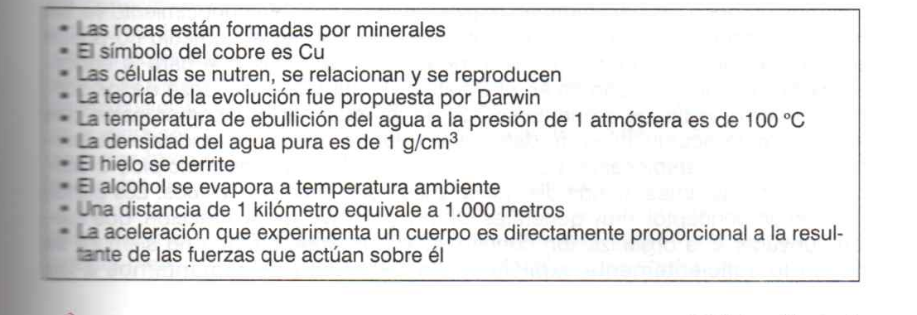
\includegraphics[width=0.5\textwidth]{tabla_4_1.png}
      \caption{Ejemplos de hechos o datos que pueden aprenderse en las clases de ciencias.}
      \label{fig:figura_4_1}
  \end{figure}
  
   \item \begin{quote}
  [...] una cosa es tener un dato, conocer algo como un hecho y otra darle sentido o significado. Comprender un dato requiere utilizar \textit{conceptos}, es decir, relacionar esos datos dentro de una red de significados que explique por qué se reproducen y qué consecuencias tienen. Los bebés saben que los objetos no soportados caen, pero otra cosa es que sepan interpretar ese hecho. Conocer un dato permite, en el mejor de los casos, reproducirlo (un número de teléfono o la masa atómica del cadmio) o predecirlo (el objeto caerá o se detendrá, esas nubes presagian lluvia esta tarde), pero no darle sentido o interpretarlo. ¿Por qué no influye la masa en la velocidad con que caen los objetos? ¿Por qué se evapora el agua? ¿Por qué es maypr la masa atómica del cobre que la del hidrógeno? \hl{(p.86)}
  \end{quote}
\end{enumerate}

\subsection*{¿Tienen que aprender datos los alumnos?}
\addcontentsline{toc}{subsection}{¿Tienen que aprender datos los alumnos?}

\begin{enumerate}
  \setcounter{enumi}{3}

  \item \begin{quote}
  Ésta es una pregunta relevante para muchos profesores, que observan cómo ciertos hechos y datos muy queridos por ellos parecen verse relegados al cajón de los contenidos obsoletos ante la creciente búsqueda de significado de todos los conocimientos. Cuando, en palabras de \textsc{García Márquez}, éramos jóvenes e indocumentados, todos nosotros tuvimos que aprender, o al menos estudiar, interminables listas, letanías de fórmulas, símbolos químicos, pero también afluentes por la derecha y por la izquierda, capitales de países remotos, la mayor parte de los cuales ya no existen. ¿Qué fue de aquel saber verbal? ¿No tiene ya sentido en nuestra sociedad? ¿No se están relegando ciertos contenidos básicos en favor de lograr otros objetivos, como la construcción de ciertos contenidos conceptuales por los alumnos, que resultan difícilmente alcanzables? \hl{(p.87)}
  \end{quote}

  \item \begin{quote}
  Hay que situar la educación científica en el contexto de una sociedad en la que \textit{sobra información} y \textit{faltan marcos conceptuales para interpretar esa información}, de modo que la transmisión de datos no debería constituir un fin principal de la educación científica, que debería estar dirigida más bien a dar sentido al mundo que nos rodea, a comprender las leyes y principios que lo rigen. \hl{(p.88)}
  \end{quote}

  \item \begin{quote}
  Enseñar los conocimientos científicos como datos, como hechos, sin significado para el alumno, axiomas o principios no entendidos ni discutidos (\textit{“la materia está compuesta de átomos separados entre sí por un espacio vacío”}, \textit{“el viento es aire en movimiento”}) convierte el aprendizaje de la ciencia en una cuestión de fe, y a los alumnos en creyentes, o más frecuentemente apóstatas, condenados al infierno de los suspensos, cuando no se quedan en el \textit{limbo} de la falta de comprensión. \hl{(p.89)}
  \end{quote}

\end{enumerate}

\subsection*{La comprensión de conceptos: aprendizaje significativo y conocimientos previos}
\addcontentsline{toc}{subsection}{La comprensión de conceptos: aprendizaje significativo y conocimientos previos}

\begin{enumerate}
  \setcounter{enumi}{6}

  \item \begin{quote}
  Una persona adquiere un concepto cuando es capaz de dotar de significado a un material o una información que se le presenta, es decir cuando “comprende” ese material; donde comprender sería equivalente, más o menos, a traducir algo a las propias palabras. \hl{(p.89)}
  \end{quote}

  \item \begin{quote}
  Un problema muy habitual en nuestras aulas es que los profesores “explican” o enseñan “conceptos” (la energía cinética, el enlace covalente, la fotosíntesis o la densidad) que los alumnos en realidad aprenden como una lista de datos, que se limitan a memorizar o reproducir en el mejor de los casos. Esto se debe a que la comprensión es más exigente para el alumno que la mera repetición. \hl{(p.90)}
  \end{quote}
  
  \item \begin{quote}
  Todos estos rasgos hacen que el aprendizaje de conceptos sea más eficaz y duradero que el aprendizaje de datos, pero también más exigente. Sus resultados son mejores, pero las condiciones para que se ponga en marcha son también más difíciles. Como mostró \textsc{Ausubel} en su teoría sobre el aprendizaje significativo (\textsc{Ausubel, Novak y Hanesian}, 1978), deben cumplirse ciertas condiciones para que tenga lugar la comprensión (véase Figura~\ref{fig:figura_4_1}). \hl{(p.92)}
  \end{quote}

  \begin{figure}[H]
      \centering
      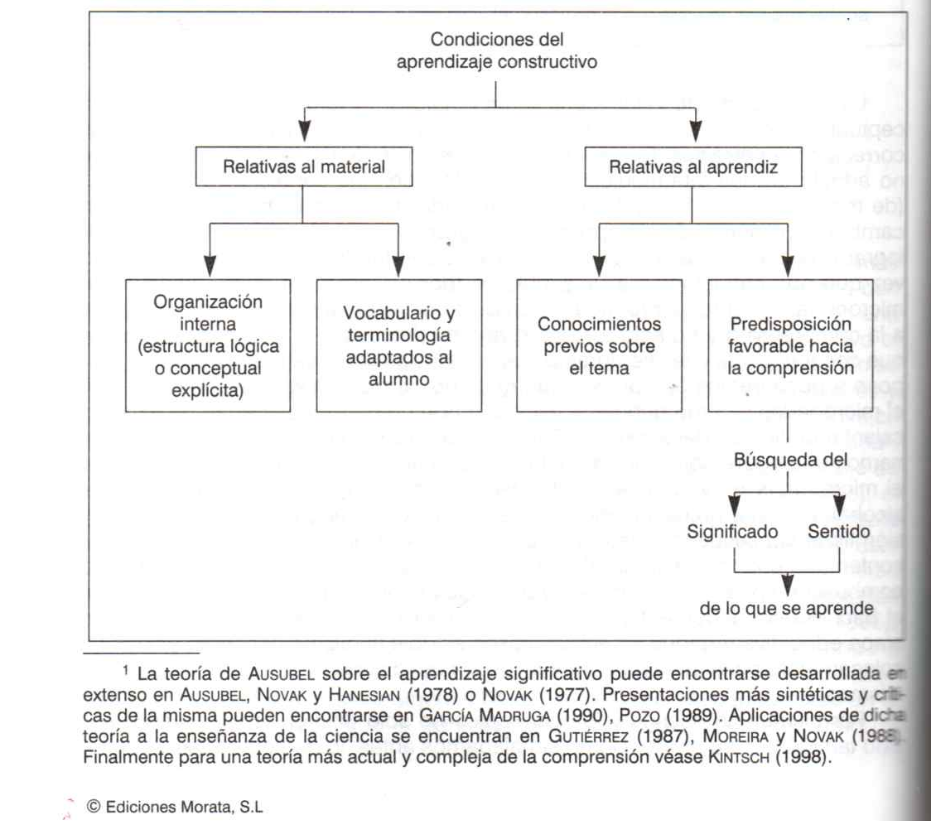
\includegraphics[width=0.5\textwidth]{figura_4_1.png}
      \caption{Condiciones o requisitos para que se produzca un aprendizaje constructivo (según \textsc{Ausubel, Novak y Hanesian}, 1978).}
      \label{fig:figura_4_1}
  \end{figure}
  
    \item \begin{quote}
  Comenzando por las características que debe tener el material de aprendizaje para que pueda ser comprendido, la principal exigencia es que tenga una organización conceptual interna, es decir, que no constituya una lista arbitraria de elementos yuxtapuestos. \hl{(p.93)}
  \end{quote}
\end{enumerate}

\subsection*{El origen de las concepciones alternativas}
\addcontentsline{toc}{subsection}{El origen de las concepciones alternativas}

\begin{enumerate}
  \setcounter{enumi}{10}

  \item \begin{quote}
  Las concepciones alternativas no son un problema más, sino otra manifestación del mismo problema, que tiene dimensiones actitudinales, procedimentales y conceptuales: la desconexión entre el conocimiento que los alumnos generan para dar sentido al mundo que les rodea, un mundo de objetos y personas, y el conocimiento científico, plagado de extraños símbolos y conceptos abstractos referidos a un mundo más imaginario que real. Mientras que el conocimiento conceptual que los alumnos traen al aula, y con él sus actitudes y procedimientos, se refiere al mundo cotidiano, un \textit{mesocosmos} trazado por las coordenadas espacio–temporales del aquí y ahora, la ciencia que se les enseña se mueve más en la “realidad virtual” del \textit{microcosmos} (células, partículas y otras entidades mágicas y no observables) y del \textit{macrocosmos} (modelos idealizados, basados en leyes universales, no vinculados a realidades concretas, cambios biológicos y geológicos que se miden en miles, si no millones de años, sistemas en interacción compleja, etc.). \hl{(p.97)}
  \end{quote}
\end{enumerate}

\subsection*{Origen sensorial: las concepciones espontáneas}
\addcontentsline{toc}{subsection}{Origen sensorial: las concepciones espontáneas}

\begin{enumerate}
  \setcounter{enumi}{11}
\item \begin{quote} Buena parte de esas concepciones alternativas se formarían, de modo espontáneo, en el intento de dar significado a las actividades cotidianas y se basarían esencialmente en el uso de reglas de inferencia causal aplicadas a datos recogidos —en el caso del mundo natural— mediante procesos sensoriales y perceptivos. Cada vez que nos enfrentamos a un suceso nuevo, o sea, moderadamente discrepante de nuestras expectativas, iniciamos una búsqueda causal con el fin de encontrar información que nos permita predecir y controlar ese suceso. \hl{(p.98)}
\end{quote}
\end{enumerate}

% (Opcional) Tabla del subcapítulo
\begin{figure}[H]
  \centering
  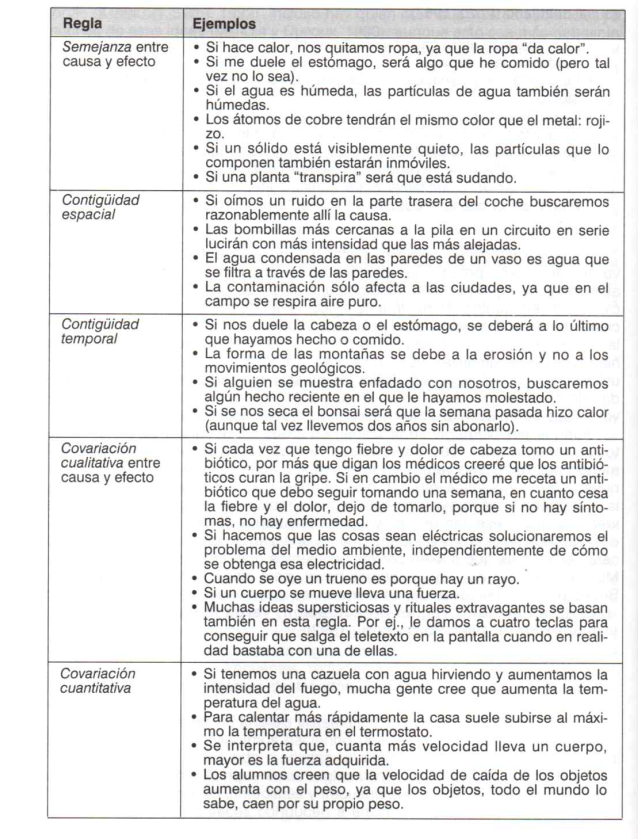
\includegraphics[width=0.5\textwidth]{tabla_4_4.png}
  \caption{Algunos ejemplos de la utilización de heurísticos o reglas simplificadoras en la formación de las concepciones espontáneas (Tabla 4.4, p.~100).}
  \label{fig:tabla_4_4}
\end{figure}

\subsection*{Origen cultural: las representaciones sociales}
\addcontentsline{toc}{subsection}{Origen cultural: las representaciones sociales}

\begin{enumerate}
  \setcounter{enumi}{12}
  \item \begin{quote}
  A diferencia de las reglas que acabamos de analizar, estas concepciones tendrían su origen no tanto en la interacción directa, sensorial, con el mundo, como en el entorno social y cultural, de cuyas ideas se impregnaría el alumno. La cultura es, entre otras muchas cosas, un conjunto de creencias compartidas por unos grupos sociales, de modo que la educación y la socialización tendrían entre sus metas prioritarias la asimilación de esas creencias por parte de los individuos. Dado que el sistema educativo no es hoy el único vehículo —y a veces ni siquiera el más importante— de transmisión cultural, los alumnos accederían a las aulas con creencias socialmente inducidas sobre numerosos hechos y fenómenos. Hay ciertos modelos, como el modelo de contagio en la transmisión de enfermedades, o los modelos de gasto y consumo (de energía, de recursos naturales, etc.), que \textit{aparecen de modo recurrente en nuestra cultura}, bien por transmisión oral, bien por su presentación a través de los medios de comunicación, que en la sociedad de la información desempeñan una función cada vez más relevante en la \textit{difusión} de ciertas concepciones alternativas, ya sea en su intento de divulgación, o incluso a través de la publicidad que nos ofrece detergentes con \textit{bioalcohol} o refrigeradores con \textit{frigofrías}. \hl{(p.101)}
  \end{quote}
\end{enumerate}


\subsection*{Origen escolar: las concepciones analógicas}
\addcontentsline{toc}{subsection}{Origen escolar: las concepciones analógicas}

\begin{enumerate}
  \setcounter{enumi}{13}
  \item \begin{quote}
  Cuando se habla de las ideas de los alumnos suele pensarse implícitamente en las dos fuentes que acabamos de mencionar, olvidándose con frecuencia la importancia de los aprendizajes escolares en la generación de ideas que van a influir a su vez en posteriores aprendizajes. Únicamente se suele hacer mención a esta fuente para referirse a posibles “errores” conceptuales de los alumnos que \textit{tienen aparentemente su origen en la propia enseñanza recibida}. Presentaciones deformadas o simplificadas de ciertos conceptos conducen a una comprensión errónea, desviada, por parte de los alumnos que no hace sino reflejar la información o la interpretación recibida. \hl{(p.102–103)}
  \end{quote}
\end{enumerate}


\subsection*{Las concepciones alternativas como teorías implícitas}
\addcontentsline{toc}{subsection}{Las concepciones alternativas como teorías implícitas}

\begin{enumerate}
  \setcounter{enumi}{14}
  \item \begin{quote}
  En suma, las concepciones alternativas no son algo accidental o coyuntural sino que tienen una naturaleza \textit{estructural}, sistemática. Son el resultado de una mente o un sistema cognitivo que intenta dar sentido a un mundo definido no sólo por las relaciones entre los objetos físicos que pueblan el mundo, sino también por las relaciones sociales y culturales que se establecen en torno a esos objetos. No es extraño por tanto que resulte tan difícil desembarazarse de ellas en la enseñanza, ya que conforman buena parte de nuestro \textit{sentido común} e incluso de nuestra tradición cultural. \hl{(p.103–109)}
  \end{quote}
\end{enumerate}

\begin{figure}[H]
  \centering
  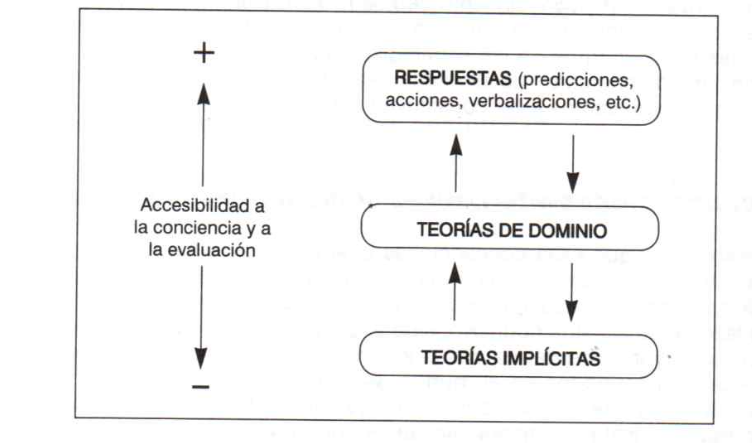
\includegraphics[width=0.5\textwidth]{figura_4_2.png}
  \caption{Niveles de análisis de las representaciones (Figura 4.2, p.~104).}
  \label{fig:figura_4_2}
\end{figure}

\begin{figure}[H]
  \centering
  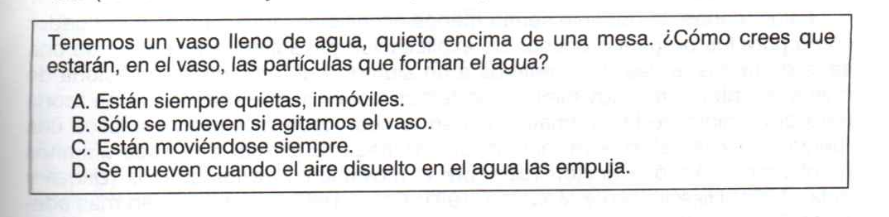
\includegraphics[width=0.5\textwidth]{tabla_4_5.png}
  \caption{Ejemplo de ítem de química para estudiar las creencias de los alumnos sobre el movimiento de partículas (Tabla 4.5, p.~105).}
  \label{fig:tabla_4_5}
\end{figure}

\subsection*{Principios epistemológicos}
\addcontentsline{toc}{subsection}{Principios epistemológicos}

\begin{enumerate}
  \setcounter{enumi}{15}
  \item \begin{quote}
  Según \textsc{Vosniadou} (1994a), entre las teorías científicas y las teorías de dominio mantenidas por los sujetos existe una incompatibilidad básica debida a ciertos supuestos epistemológicos impuestos por la \textit{teoría–marco}, o \textit{teoría implícita}, al sistema de creencias de los alumnos, que no serían compatibles con los supuestos subyacentes a la teoría científica. Estos supuestos tendrían una función similar en el conocimiento cotidiano a las paradigmas de \textsc{Kuhn} (1962) o a los programas de investigación de \textsc{Lakatos} (1978). Es decir que, a la hora de generar representaciones específicas para predecir o explicar cualquier fenómeno cotidiano, nuestro conocimiento intuitivo \textit{asume} de forma implícita ciertos principios sobre la naturaleza de la realidad y actúa conforme a ellos. \hl{(p.109–111)}
  \end{quote}
\end{enumerate}

\begin{figure}[H]
  \centering
  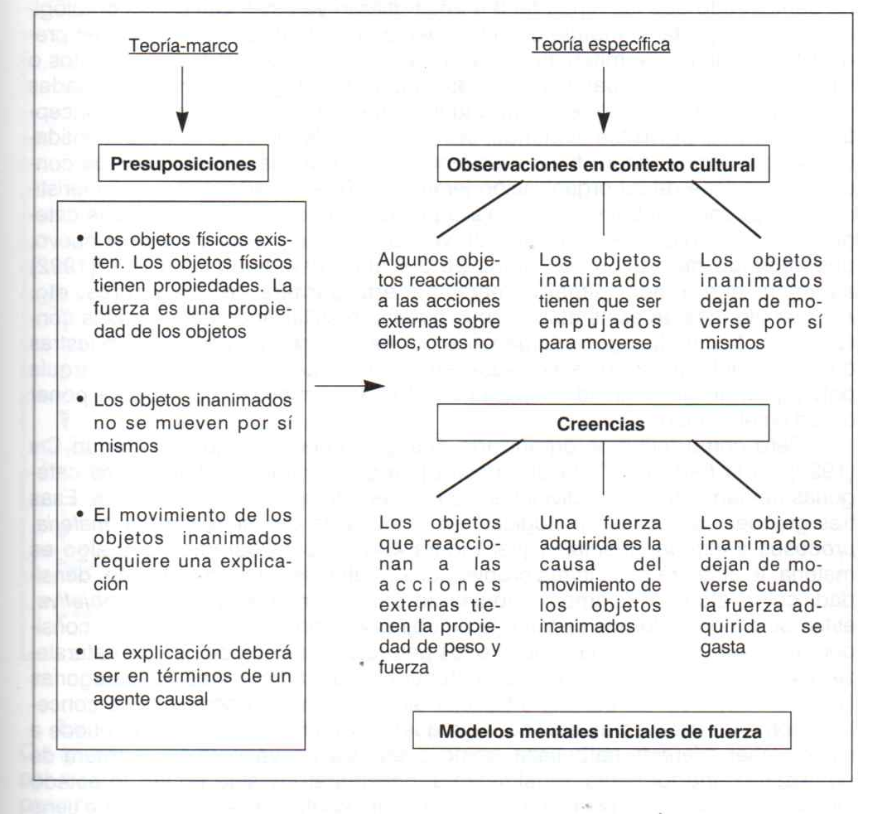
\includegraphics[width=0.5\textwidth]{figura_4_3.png}
  \caption{Estructura conceptual hipotética que subyace a los modelos mentales iniciales de fuerza según \textsc{Vosniadou} (1994a) (Figura 4.3, p.~111).}
  \label{fig:figura_4_3}
\end{figure}

\subsection*{Principios ontológicos}
\addcontentsline{toc}{subsection}{Principios ontológicos}

\begin{enumerate}
  \setcounter{enumi}{16}
  \item \begin{quote}
  Otra teoría del cambio conceptual, desarrollada por \textsc{Chi} (1992; \textsc{Chi, Slotta y de Leeuw}, 1994), propone unos rasgos más precisos y detallados, al concebir que el cambio conceptual se hace necesario cuando existe una incompatibilidad ontológica entre la teoría científica y la teoría mantenida por el alumno. Según este modelo, las personas clasificamos todos los objetos del mundo en un número limitado de categorías ontológicas, a las que atribuimos unas propiedades determinadas. Cada vez que interpretamos que un hecho o un objeto pertenece a una determinada categoría ontológica (es una enfermedad, un proceso de evaporación o un pájaro), por el simple hecho de categorizarlo así, tendemos a atribuirle una serie de características. \hl{(p.111–115)}
  \end{quote}
\end{enumerate}

\begin{figure}[H]
  \centering
  \includegraphics[width=0.85\textwidth]{figura_4_4.png}
  \caption{Un posible esquema de categorización del mundo según \textsc{Chi} (1992). Las categorías separadas en forma horizontal son ontológicamente diferentes; el cambio conceptual implica el paso de una rama principal a otra (Figura 4.4, p.~113).}
  \label{fig:figura_4_4}
\end{figure}

\subsection*{Principios conceptuales}
\addcontentsline{toc}{subsection}{Principios conceptuales}

\begin{enumerate}
  \setcounter{enumi}{17}
  \item \begin{quote}
  Una diferencia esencial entre las teorías cotidianas y científicas reside en la forma en que están estructurados los conceptos en unas y otras. Mientras que las teorías científicas utilizan \textit{esquemas o estructuras conceptuales} próximos a los esquemas operatorios formales de \textsc{Inhelder} y \textsc{Piaget} (1955), las teorías implícitas se basan en estructuras conceptuales más simples, que se oponen en buena medida a los esquemas formales subyacentes a las teorías científicas. 
  Por ello, el aprendizaje de la ciencia requiere, además del cambio epistemológico y ontológico, un cambio en las estructuras conceptuales, o \textit{reestructuración de los conocimientos}. \hl{(p.~115–119)}
  \end{quote}
\end{enumerate}

\begin{table}[H]
\centering
\caption{Restricciones estructurales de las teorías implícitas frente al conocimiento formal o científico (Tabla 4.6).}
\begin{tabular}{|p{6cm}|p{6cm}|}
\hline
\textbf{RESTRICCIONES ESTRUCTURALES (Teorías implícitas)} & 
\textbf{ESQUEMAS FORMALES (Teorías científicas)} \\ \hline
Causalidad lineal y simple en un solo sentido (agente $\rightarrow$ objeto) & 
Interacción de sistemas, causalidad compleja \\ \hline
No cuantificación o estrategias de cuantificación erróneas & 
Proporción, probabilidad, correlación \\ \hline
Transformación sin conservación & 
Conservaciones no observables, sistemas en equilibrio \\ \hline
\end{tabular}
\end{table}

\paragraph{a) Causalidad lineal frente a interacción de sistemas}
Los alumnos tienden a recurrir a un esquema causal simple donde la relación causa–efecto es lineal y unidireccional. En cambio, las teorías científicas requieren comprender las situaciones como interacciones de sistemas en las que intervienen múltiples causas coordinadas. Esta diferencia es clave para entender principios como la conservación de la energía o la estructura corpuscular de la materia.

\paragraph{b) Cambio y transformación frente a conservación y equilibrio}
Las teorías implícitas suelen centrarse en el cambio visible, descuidando lo que se conserva. Las teorías científicas, por el contrario, se organizan en torno a sistemas de equilibrio y conservación —ya sean mecánicos, físicos, químicos o ecológicos—, que implican comprender la estabilidad dinámica subyacente a los fenómenos.

\paragraph{c) Relaciones cualitativas frente a esquemas de cuantificación}
El pensamiento cotidiano establece relaciones cualitativas sin cuantificar. La ciencia, en cambio, exige cuantificación precisa mediante los esquemas de \textbf{proporción}, \textbf{probabilidad} y \textbf{correlación}. Estos esquemas, poco intuitivos, requieren una reestructuración cognitiva avanzada.

\begin{quote}
En suma, las teorías científicas difieren del conocimiento cotidiano tanto en las relaciones cualitativas (conservación, equilibrio, interacción sistémica) como en las cuantitativas (proporción, probabilidad, correlación). Este cambio conceptual implica adquirir nuevas estructuras conceptuales estrechamente ligadas a los principios epistemológicos y ontológicos previos. 
\end{quote}

\setcounter{enumi}{18}
\subsection*{De las teorías implícitas a las teorías científicas: ¿qué cambia en el cambio conceptual?}
\addcontentsline{toc}{subsection}{De las teorías implícitas a las teorías científicas: ¿qué cambia en el cambio conceptual?}

\begin{enumerate}
  \setcounter{enumi}{18}
  \item \begin{quote}
  Como hemos ido viendo, si asumimos que las “concepciones alternativas” son de algún modo el resultado del “sentido común” —es decir el funcionamiento del sistema cognitivo humano como producto biológico y cultural— aplicado a la predicción y control de los fenómenos científicos, cambiar esas concepciones alternativas requiere algo más que sustituir las ideas de los alumnos por otras científicamente más aceptables. Requiere de hecho modificar sustancialmente los principios en los que está basado, de modo implícito, ese procesamiento y ese conocimiento. Requiere en suma \textit{reformatear} la mente de los alumnos o al menos incorporarle un nuevo sistema operativo que sea compatible con los principios en que se basa el conocimiento científico. \hl{(p.~119)}
  \end{quote}
\end{enumerate}

\begin{table}[H]
\centering
\caption{Tres dimensiones de cambio en el aprendizaje de la ciencia (Tabla 4.7).}
\begin{tabular}{|p{4.8cm}|p{4.8cm}|p{4.8cm}|}
\hline
\multicolumn{3}{|c|}{\textbf{PRINCIPIOS EPISTEMOLÓGICOS}} \\ \hline
\textbf{Realismo ingenuo} & \textbf{Realismo interpretativo} & \textbf{Constructivismo} \\ \hline
\textit{La realidad es tal como la vemos. Lo que no se percibe no se concibe.} &
\textit{La realidad existe y tiene sus propiedades, aunque no siempre podamos conocerla directamente, pero mediante la ciencia y la técnica podemos saber cómo es realmente.} &
\textit{El conocimiento científico es una construcción que nos proporciona modelos alternativos para interpretar la realidad, pero que no son parte de la realidad.} \\ \hline
\end{tabular}
\end{table}

% ——— Subcapítulo final ———
\subsection*{Cambio epistemológico, ontológico y en las estructuras conceptuales}
\addcontentsline{toc}{subsection}{Cambio epistemológico, ontológico y en las estructuras conceptuales}

\begin{enumerate}
  \setcounter{enumi}{19}
  \item \begin{quote}
  \textbf{Cambio epistemológico.} En el conocimiento cotidiano solemos asumir un \textit{realismo} según el cual el mundo es tal como se percibe; aprender sería copiar la realidad. En cambio, desde una posición \textit{constructivista}, el conocimiento científico consiste en \textit{elaborar modelos alternativos} para interpretarla \hl{(p.~121–123)}

  \textbf{Cambio ontológico.} El realismo ingenuo reduce los fenómenos a \textit{estados} desconectados. El progreso conceptual requiere reatribuirlos primero a \textit{procesos} y, finalmente, comprenderlos como \textit{sistemas} de relaciones en equilibrio \hl{(p.~123–125)}

  \textbf{Cambio en las estructuras conceptuales.} Se pasa de \textit{hechos} y \textit{causalidad lineal} (agente $\rightarrow$ objeto) a \textit{interacción múltiple} y conservación/equilibrio, sustituyendo reglas heurísticas por \textit{relaciones cuantitativas} (proporción, probabilidad, correlación) \hl{(p.~125–126)}
  \end{quote}
\end{enumerate}


 

\end{document}
